\subsection{可度量化拓扑空间}

定义 3. 集合 X 上的度量称为与 X 上的拓扑 C 相容，如果由该度量定义的拓扑与 C 重合。拓扑空间称为可度量化的，如果存在 X 上的一个度量与 X 的拓扑相容。

\pandocbounded{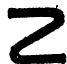
\includegraphics[keepaspectratio]{images/part001_d7e316f7.jpg}}

集合 X 上都与同一个拓扑 \(\mathfrak{C}\) 相容的两个度量可以不等价。

R 的子空间 \(R_{+}^{*}\) 提供了这样的一个例子。由 R 的加法一致结构诱导的一致结构与由 \(R^{*}\) 的乘法一致结构诱导的一致结构都是可度量化的，并且都与 \(R_{+}^{*}\) 的拓扑相容；但它们不可比较。

我们还指出，可以存在与可度量化拓扑空间的拓扑相容的不可度量化的一致结构（习题 7）。

这里我们只满足于给出拓扑空间可度量化的必要条件（关于必要充分条件，参看第 4 节，习题 22）。首先，一个空间除非是完全正则的，否则不可能是可度量化的（事实上我们将在第 4 节，第 1 号，命题 2 中看到，可度量化空间必然是``正规''的，这是一个更强的条件）。另一方面，定理 1 表明：

命题 6. 可度量化空间的每个点都具有可数的基本邻域系。

更一般地：

命题 7. 在可度量化空间中，每个闭集都是可数个开集之交，每个开集都是可数个闭集之并。

设 \(d\) 是与可度量化空间 \(\mathbf{X}\) 的拓扑相容的一个度量。若 \(\mathbf{A}\) 是 \(\mathbf{X}\) 的闭子集，则它是诸开集 \(\mathrm{V}_{1/n}(\mathbf{A})\) {[}由所有点 \(x\in\mathbf{X}\) （满足 \(d(x,\mathbf{A})<\mathbf{1}/n\) ）组成的集；参看命题 2{]}之交。命题的第二部分通过取余集得到。

注。1) 这些必要条件不是充分的（参看习题 13）。2) 存在这样的空间：其中每个点都有可数的基本邻域系，但其中存在不是可数个开集之交的闭集（习题 15）；这样的空间不是可度量化的。

第 4 节定理 1 的推论 2 表明，可度量化拓扑空间的可数乘积是可度量化的。此外，可度量化空间的任意族 \((\mathbf{X}_t)_{t \in \mathbf{I}}\) 的和 X （第一章，§ 2，第 4 号）也是可度量化的。因为若 \(d_t\) 是与 \(\mathbf{X}_t\) 的拓扑相容的度量（对每个 \(t \in \mathbf{I}\) ），则我们可以假定 \(d_t\) 有界且 \(\mathbf{X}_t\) 的直径 \(\leqslant t\) ；于是可以定义一个距离 \(d\) （与 \(\mathbf{X}\) 的拓扑相容）：规定 \(d(x, y) = d_t(x, y)\) 当 \(x\) 与 \(y\) 都属于同一个 \(\mathbf{X}_t\) 时，否则规定 \(d(x, y) = t\) 。

